\documentclass[a4, 11pt]{article}
\usepackage[utf8]{inputenc}
\usepackage[a4paper,bindingoffset=0.2in,%
 left=1in,right=1in,top=1in,bottom=1in,%
            footskip=.25in]{geometry}
\usepackage{cite}
\usepackage[english]{babel}
\usepackage{graphicx}
\usepackage{caption}
\usepackage{subfigure}
\usepackage{hyperref}
\setlength{\parskip}{1em}
\renewcommand{\baselinestretch}{1.0}
\setlength{\parindent}{0pt}

\title{%
  COMP20008 Assignment 2 \\
  \large Data Science Project Report\\
  }
\author{Steven Nguyen, Lina Zhu, Sen Turner}
\date{}


\begin{document}
\maketitle
\section{Introduction}

In this report we examine how childhood developmental factors and experiences in school-aged individuals affect the prevalence of depression in young-adults. By examining this we aim to identify and isolate external childhood developmental factors that may impact on the health and wellbeing of our communities. Our focus on childhood and youth development also allows us to understand the liveability of Victorian communities, as we will potentially be able to identify areas that need improved living conditions for young people.

\subsection{Data Sets Used}

To answer our question we focused on multiple datasets; the Victorian Public Health Survey, VCAMS (Victorian Child and Adolescent Monitoring System), AEDC (Australian Early Development Census) and the Education State. These allow us to examine a variety of factors influencing school aged individuals, aggregated by region. 

\begin{figure}[h]
    \centering
    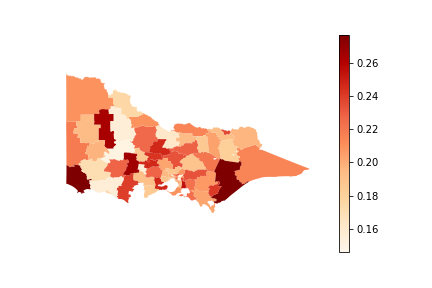
\includegraphics[width=0.6\textwidth]{./plots/depressionMap.png}
    \caption{Depression rate in young adults in Victoria by LGA}
    \label{fig:my_label}
\end{figure}

The Victorian Public Health Survey collects information about the health and wellbeing of adult Victorians, including the percentage of \emph{young adults (aged 18-25) that have ever been diagnosed with depression}, which we will refer to as `Depression rate' throughout this report. VCAMS tracks and measures a variety of indicators for young people’s health, wellbeing, safety and learning. The AEDC dataset focuses on the development of children across Australia, recording the proportion of children that are developmentally at risk or vulnerable. The Education State dataset is focused on the Victorian school system, including data surrounding the number of enrollments, teachers and expulsions. We chose factors that we believe substantially impact the liveability for school-aged individuals and potentially have a lasting mental impact, such as occurrences of bullying, access to mental health services, and so on \footnote{More information about the factors used and their definitions can be found in the README  \href{https://github.com/COMP20008/assignment-2-team55}{here}.}.  

\section{Wrangling and Analysis Methods}
Because we use a variety of data sets, there were many data files we needed to process and collect into one table for further analysis.

\begin{figure}[h]
    \centering
    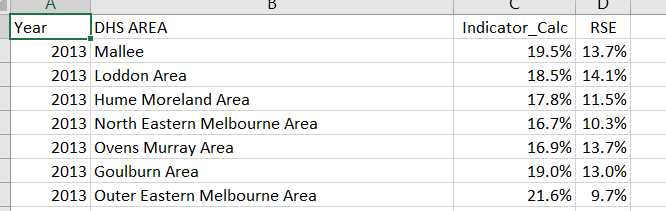
\includegraphics[width=0.5\textwidth]{./plots/conforming.png}
    \caption{Example structure of a VCAM spreadsheet.}
    \label{fig:my_label}
\end{figure}

One example issue we found was that in the VCAMs data sets, we found that while most files had a regular tabular format, a few files had differing column names or extra columns that made it harder to use the same function. 

\begin{figure}[h]
    \centering
    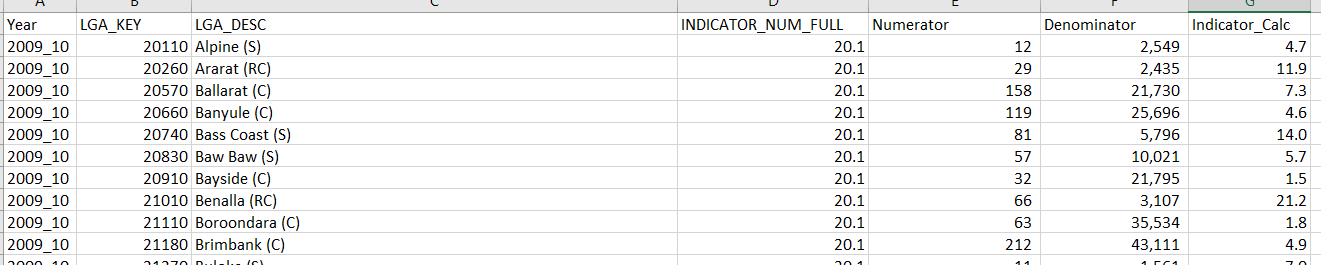
\includegraphics[width=0.9\textwidth]{./plots/nonconforming.png}
    \caption{Example of a nonconforming VCAM spreadsheet.}
    \label{fig:my_label}
\end{figure}

Some other issues included -

\begin{itemize}
    \item \verb|.pdf| format data.
    \item Inconsistent area names. (`Greater Melbourne' vs `Greater Melbourne \textit{Area}')
    \item Non-numeric or missing data which had to be imputed.
    \item Teacher data being improperly split for Catholic schools (requiring collation of secondary and primary school data)
\end{itemize}

We used a combination of manual cleaning via Excel where it was trivial to do so or not worth automating, and Python for more automated cleaning, particularly for the VCAMs datasets of which there were many.

Data sets were linked together by merging features over common keys – either LGAs (Local Government Areas) or DHS (Department of Health Services) Areas together with respective depression rates in young people for each region. It was not of interest to aggregate LGA areas into DHS areas to combine the data sets as that would result in less data points in our plots which could potentially make us lose some information. 

Data was then analysed by searching for correlations between depression rate and our chosen features in order to see whether or not youth experiences dictate future depression rates in adulthood. We also wanted to see whether or not childhood features were correlated with each other to see if there were any underlying systemic issues. To achieve this we made a pairs plot between all the relevant features initially to see if there were any correlations at all in order to guide further study. We then calculated pairwise correlation coefficients and mutual information scores, and used a variety of visualisation tools on our data. 

It was also of interest to see which LGA areas were `most liveable’ overall for youth. This was done by first doing min-max normalisation over each column. For each LGA we then took the average of these as a rough index for the youth liveability in that area, based on the given features. The higher the score, the better the region performs \emph{relative} to other LGAs in Victoria. Clustering was then done using K-means to identify and better classify low and high scoring contiguous areas. 


\newpage
\section{Results}
\subsection{Correlation}
Through our Pearson Correlation Coefficient heatmap we found overall low Pearson correlation values between rate of depression and individual childhood factors, suggesting minimal linear correlation. This was also demonstrated by our mutual information map. However, the heat maps highlight some clear linear correlations between childhood factors, particularly the AEDC indicators as well as bullying rate and connectedness to school.

\begin{figure}[h]
    \captionsetup[subfigure]{labelformat=empty}
    \centering
    \subfigure[Correlation Coefficient Heatmap]{
    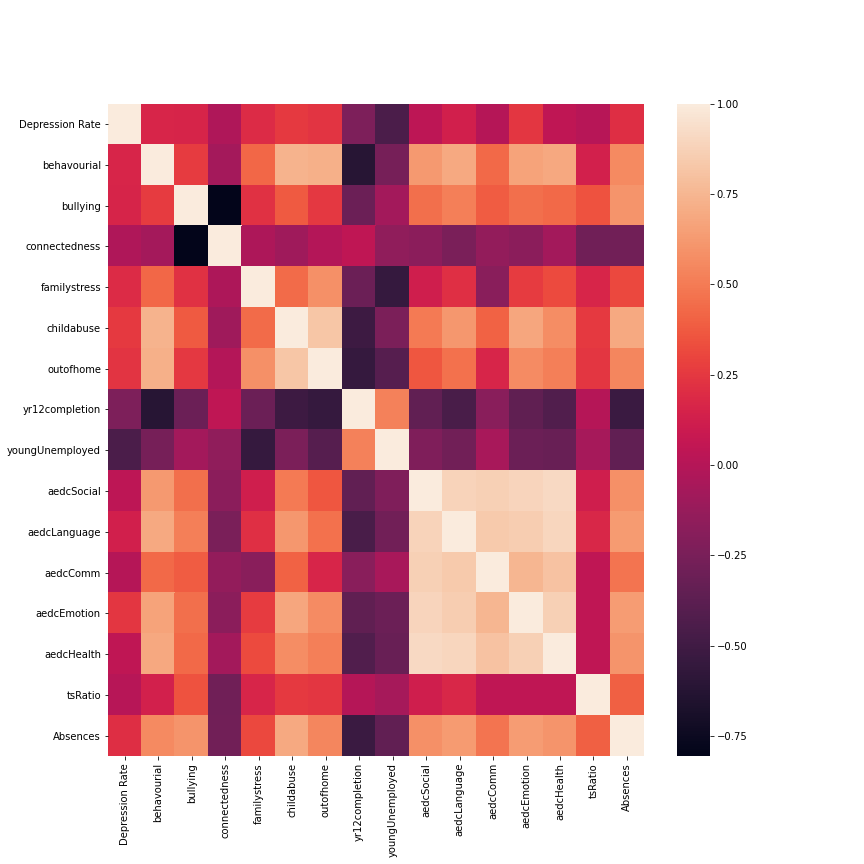
\includegraphics[width=0.45\textwidth]{./plots/correlationMap.png}
    }
    \subfigure[Mutual Information Heatmap]{
    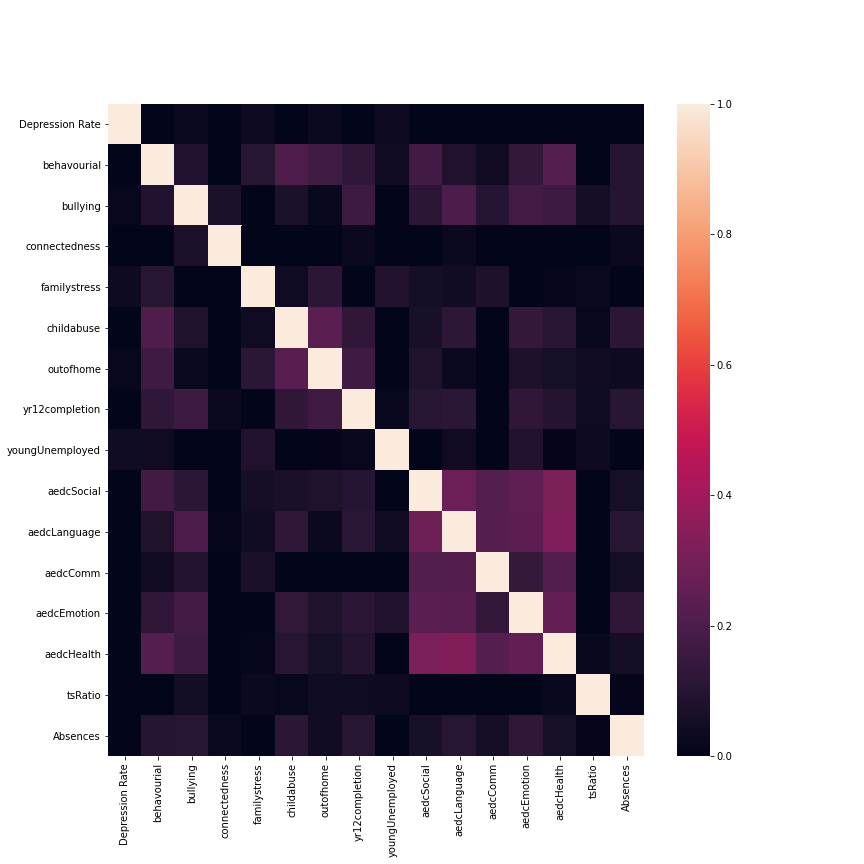
\includegraphics[width=0.45\textwidth]{./plots/midfMap.png}
    }
    \caption{Pairwise correlation matrix heatmap plots.}
\end{figure}
The low correlation between depression and childhood factors was largely to be expected, as depression is caused by a multitude of factors and can’t be expected to be linearly mapped by any individual variable. Thus, even small correlations are of interest. Rate of absences had the largest mutual information score of 0.1187, while rate of children at risk of development emotionally had the largest Pearson value, suggesting these are the features with highest correlation to depression. The relationships between these factors and depression are visualised below.

\begin{figure}[ht]
    \centering
    \begin{minipage}[b]{0.46\linewidth}
        \centering
        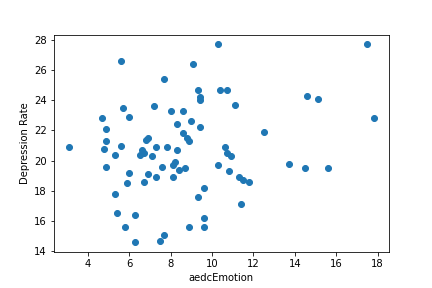
\includegraphics[width=0.9\linewidth]{./plots/depression/aedcEmotion.png}
        \caption{Depression rate vs \% of children developmentally at risk emotionally.}
        \label{fig:minipage1}
    \end{minipage}
    \quad
    \begin{minipage}[b]{0.46\linewidth}
        \centering
        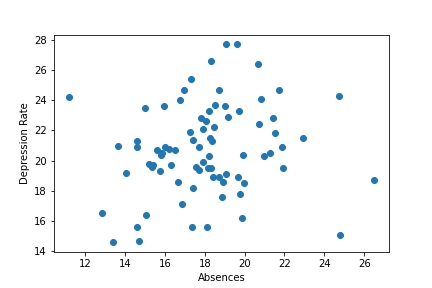
\includegraphics[width=0.9\linewidth]{./plots/depression/Absences.png}
        \caption{Depression rate vs abesences per 1000 students.}
        \label{fig:minipage2}
    \end{minipage}
\end{figure}

Visually there is a slight positive relationship between absences and depression. However, it is difficult to identify whether this is a result of early onset depression influencing absences or absences increasing susceptibility to depression. Overall, it was difficult to say from these visualisations whether there are any worthwhile correlations between depression rates and any individual factors.

Through our parallel coordinate plots we were able to visually identify some strong linear correlations within factors - for example bullying, family stress and connectedness, as seen below. This potentially suggests that high levels of family stress or children lacking connection leads to increased bullying in schools. Low, medium and high in this plot refers to low, medium and high rates of depression in each LGA (which are represented by a single line).

\begin{figure}[h]
    \centering
    
\includegraphics[width=0.6\textwidth]{./plots/parallel2.png}
    \caption{A section of a parallel plot between all the LGA features.}
    \label{fig:my_label}
\end{figure}


According to the pair plot of dhsData, the overall correlation is relatively low, making it difficult to identify any causal relationships between any of the factors. In general, positive correlation can be seen between factors that both contribute to positive impact (mental health access vs physical activities) or negative impact (psychological (stress) vs cyberbullying) on individuals. However the more interesting correlation between cyberbullying and depression rate shows a weak negative correlation which conflicts with expectation. 

\begin{figure}[h]
    \captionsetup[subfigure]{labelformat=empty}
    \centering
    \subfigure{
    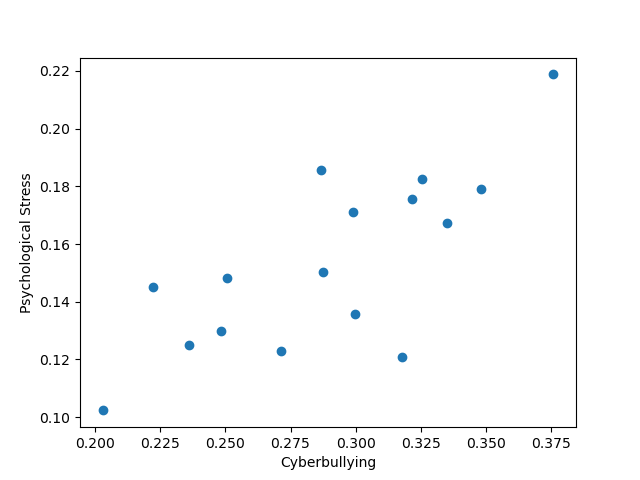
\includegraphics[width=0.30\textwidth]{./plots/cyberPsych.png}
    \label{}
    }
    \subfigure{
    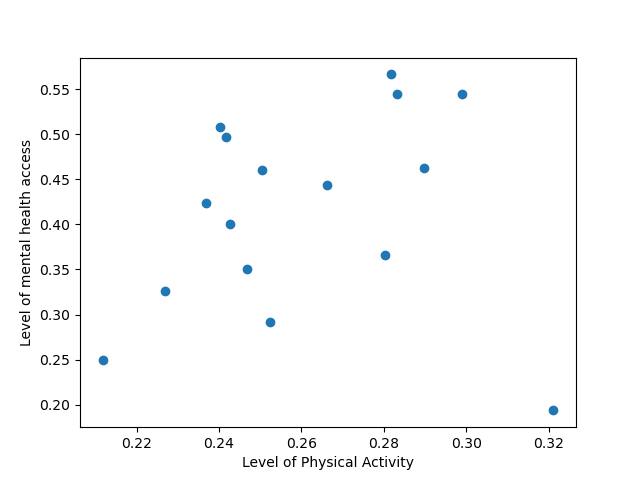
\includegraphics[width=0.30\textwidth]{./plots/mentalaccess.png}
    \label{}
    }
    \subfigure{
    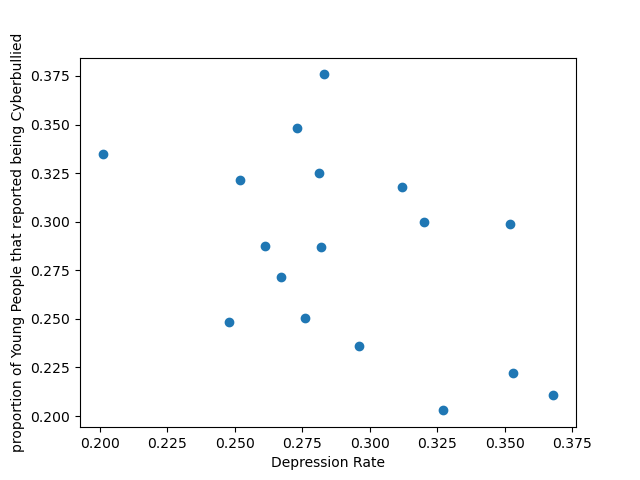
\includegraphics[width=0.30\textwidth]{./plots/cyberDepression.png}
    \label{}
    }
    \caption{Comparison of DHS Data plots.}
\end{figure}

\newpage
\subsection{Youth Liveability Index}
With our normalised ‘youth liveability score’ and depression rates we produced separate choropleths. The visual congestion of high scoring areas in the centre of the ‘youth liveability’ map suggests that areas closer to Melbourne tend to be better for youth while more rural areas are less liveable. 

\begin{figure}[h]
    \captionsetup[subfigure]{labelformat=empty}
    \centering
    \subfigure[Youth Liveability Index Map]{
    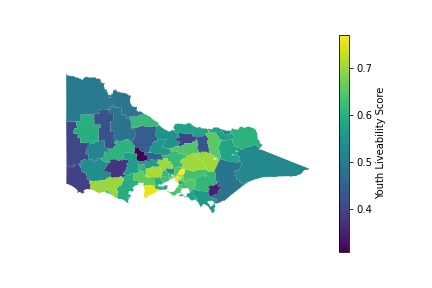
\includegraphics[width=0.47\textwidth]{./plots/scoremapminMax.png}
    }
    \subfigure[Depression Rate Map]{
    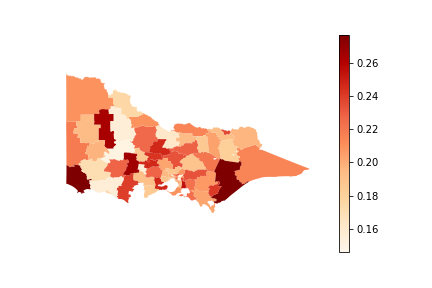
\includegraphics[width=0.47\textwidth]{./plots/depressionMap.png}
    }
    \caption{Comparison of depression rate against overall score for each region.}
\end{figure}

\begin{figure}[h]
    \centering
    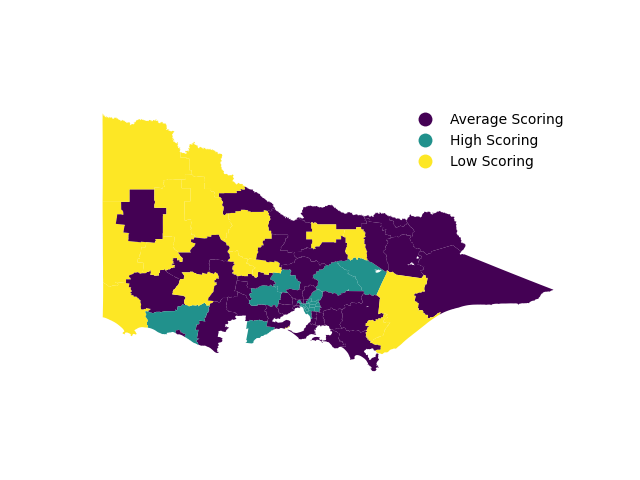
\includegraphics[width=0.8\textwidth]{./plots/kmeansminMax.png}
    \caption{Map clustered by liveability score using K-means (k=3).}
    \label{fig:my_label}
\end{figure}

We gather that there is a wide spread of areas that are performing similar, but low scoring areas tend to be concentrated in rural North Western Victoria.

\newpage

Finally, we created a scatterplot comparing liveability index and depression rate. This graph demonstrates a slight negative correlation, suggesting that increasing youth liveability may have a slight impact on decreasing depression later in life. However, the lack of strong correlation as well as high variance suggests there are more causal factors to identify than just childhood liveability.

\begin{figure}[ht]
    \centering
    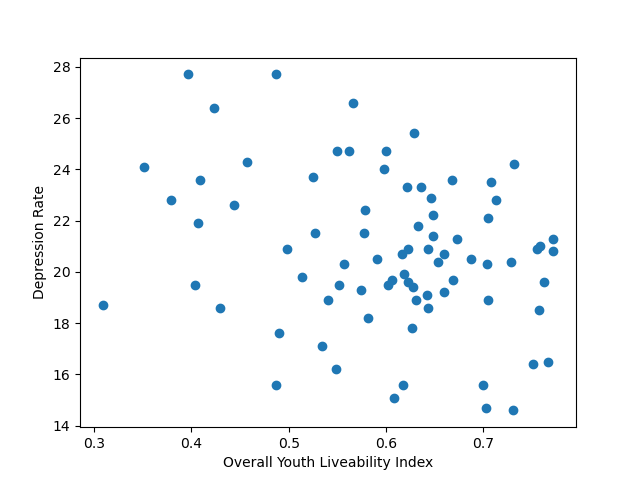
\includegraphics[width=0.6\textwidth]{./plots/overallscatterminMax.png}
    \label{fig:my_label}
\end{figure}

\subsection{Limitations}

Overall the data is not enough to conclude that there is any significant relationship between depression rate in adults and childhood factors. While there are some slight correlations that warrant further investigation there is nothing significant enough to make outright conclusions. Depression rates as seen on the map vary significantly between areas, and there are likely a lot of causes depending on the individual. Moreover, since we are simply doing an observational study of populations in an area, there is no way to account for any confounding factors - obvious ones being socioeconomic differences between rural and urban populations.

This analysis could potentially be improved by combining the DHS and LGA data through aggregation, meaning we don’t need to analyse these factors separately, or simply by analysing more features. Additionally, ideally the liveability index would have weighting introduced, as some factors are more important when considering liveability. An increased focus on this overall welfare/liveability may also improve our conclusions. It is somewhat unlikely that any individual variable significantly impacts depression, but overall child welfare is more likely to show correlation. Similarly, it would potentially benefit the analysis to place additional focus on individuals rather than sole focus on populations in specific regions.  This would allow us to look at individuals without the bias across a population in a local government area.

\section{Conclusion}


Based on the results we gathered as well as the limitations of our design, we cannot make strong conclusions as to whether depression rates and childhood factors are indeed highly correlated, despite most of the selected features influencing young individuals in a clearly negative way. However, the supplementary information gathered on liveability in regions for young, school-aged individuals is still valuable - showing a clear difference between rural and urban areas. Moreover we did find that quite a few features were highly correlated, strongly suggesting  that one issue leads to other issues in a child’s life. With this information we can pinpoint ways in order to improve young people’s lives, particularly in struggling areas. 

\subsection*{Links to Data Sets}
https://www.education.vic.gov.au/about/research/Pages/vcamsindicator.aspx  \\
https://www.aedc.gov.au/resources/detail/public-table-by-local-government-area-(lga)-2009-2018\\
https://www.education.vic.gov.au/Documents/school/teachers/profdev/careers/TSDR-2018-final-report.docx\\
https://www2.health.vic.gov.au/public-health/population-health-systems/health-status-of-victorians/
survey -data-and-reports/victorian-population-health-survey/victorian-population-health-survey-2011-12\\
https://www.bettersafercare.vic.gov.au/reports-and-publications/vphs2018 \\

\end{document}
